\documentclass[aspectratio=169,10pt]{beamer}

\usetheme{Madrid}
\usecolortheme{seahorse}

% Packages
\usepackage[utf8]{inputenc}
\usepackage{amsmath, amssymb, amsfonts}
\usepackage{graphicx}
\usepackage{xcolor}
\usepackage{listings}
\usepackage{xparse}
\usepackage{soul}

% Set graphics path
\graphicspath{{figures/}}

% Color definitions
\definecolor{codebg}{RGB}{240,240,240}
\definecolor{codegreen}{RGB}{0,128,0}

% Code listing style
\lstset{
    basicstyle=\ttfamily\small,
    commentstyle=\color{codegreen}\itshape,
    keywordstyle=\color{blue},
    stringstyle=\color{red},
    breaklines=true,
    tabsize=2,
    numberstyle=\tiny,
    numbers=left,
    frame=single,
    backgroundcolor=\color{codebg},
    language=Python
}

% Custom theorem styles
\setbeamertemplate{theorems}[numbered]
\setbeamertemplate{footline}[frame number]

% Define custom commands for math
\newcommand{\Prob}[1]{\mathbb{P}(#1)}
\newcommand{\E}[1]{\mathbb{E}[#1]}
\newcommand{\R}{\mathbb{R}}
\newcommand{\HH}{\mathcal{H}}
\newcommand{\X}{\mathcal{X}}
\newcommand{\F}{\mathcal{F}}
\newcommand{\norm}[1]{\left\|#1\right\|}
\newcommand{\abs}[1]{\left|#1\right|}
\newcommand{\inner}[2]{\langle #1, #2 \rangle}
\newcommand{\defeq}{\vcentcolon=}

% Title Page
\title{Normal Structure \& Fixed Point Theory}
\subtitle{Chapter 6c: Applications of Monotone Operator Theory}
\author{Based on Pathak's \textit{An Introduction to Nonlinear Analysis and Fixed Point Theory}}
\date{\today}
\institute{Lecture Series on Monte Carlo Theory}

\begin{document}

% Title slide
\frame{\titlepage}

% Table of contents
\begin{frame}[allowframebreaks]{Outline}
    \tableofcontents
\end{frame}

% ==================== SECTION 1: INTRODUCTION ====================
\section{Introduction: Normal Structure and Fixed Points}

\begin{frame}{What is Normal Structure?}
    \begin{definition}[Normal Structure]
        A convex set $K$ in a Banach space $X$ is said to have \textbf{normal structure} if for each bounded convex subset $H$ of $K$ that contains more than one point, there exists a point $x \in H$ that is not a diametral point of $H$.
    \end{definition}

    \vspace{0.3cm}

    \begin{itemize}
        \item A diametral point is one where the distance to the boundary equals the diameter $\delta(H)$
        \item Normal structure is a fundamental concept in fixed point theory
        \item Every compact convex set in a Banach space has normal structure (Theorem 5.27)
    \end{itemize}

    \begin{example}
        Any bounded convex set in a uniformly convex Banach space has normal structure.
    \end{example}
\end{frame}

\begin{frame}{Key Motivation}
    \begin{center}
        \Large \textbf{Central Question:}\\[0.3cm]
        When do nonexpansive and monotone mappings have fixed points?
    \end{center}

    \vspace{0.5cm}

    \textbf{Key Results:}
    \begin{enumerate}
        \item Normal structure implies existence of fixed points for certain nonexpansive mappings
        \item Kirk's theorem connects normal structure to fixed point properties
        \item Monotone operators provide powerful tools for integral equations
        \item Hammerstein equations: combining linear and nonlinear operators
    \end{enumerate}

    \vspace{0.3cm}
    This chapter bridges geometric properties (normal structure) with operator-theoretic methods.
\end{frame}

% ==================== SECTION 2: MONOTONE OPERATORS ====================
\section{Monotone Operators and Hilbert Spaces}

\begin{frame}{Monotone Operators: Definition}
    \begin{definition}[Monotone Operator]
        An operator $T: X \to X^*$ on a Banach space $X$ is \textbf{monotone} if for all $x, y \in X$:
        \[
            \langle Tx - Ty, x - y \rangle \geq 0
        \]
    \end{definition}

    \vspace{0.3cm}

    \begin{definition}[Strongly Monotone Operator]
        $T$ is \textbf{strongly monotone} with constant $c > 0$ if:
        \[
            \langle Tx - Ty, x - y \rangle \geq c\|x - y\|^2
        \]
    \end{definition}

    \vspace{0.3cm}

    \textbf{Examples:}
    \begin{itemize}
        \item Identity map $I$ is strongly monotone with $c = 1$
        \item Gradient of convex function: $\nabla f$ is monotone if $f$ is convex
        \item Integral operators with appropriate kernels
    \end{itemize}
\end{frame}

\begin{frame}{Monotone Properties}
    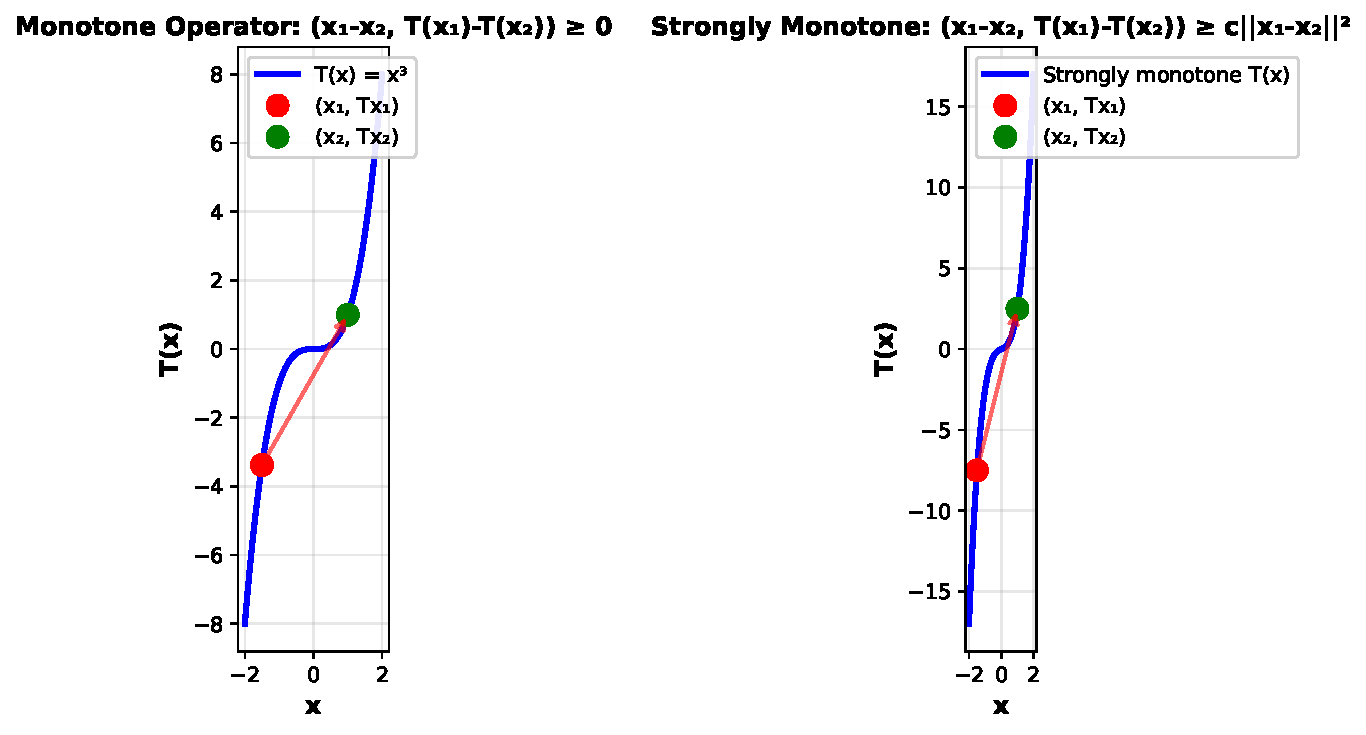
\includegraphics[width=\textwidth]{monotone_operator_property.pdf}
\end{frame}

\begin{frame}{Key Theorem: Monotone Operators with Hilbert Spaces}
    \begin{theorem}[Dolph-Minty, Theorem 8.8]
        Let $\HH$ be a Hilbert space and $N_f: \HH \to \HH$ be hemicontinuous and monotone,
        and $K: \HH \to \HH$ continuous and strongly monotone. Then:
        \begin{enumerate}
            \item Equation (8.31): $x + KN_f x = y$ has a \textbf{unique solution} $x$ for every $y$
            \item The solution depends continuously on $y$ and satisfies:
            \[
                \|x\| \leq \frac{1}{c}\|K\|\|y\|
            \]
            where $c$ is the strong monotonicity constant.
        \end{enumerate}
    \end{theorem}

    \vspace{0.3cm}
    \small
    \textbf{Proof idea:} Use strong monotonicity to establish injectivity and surjectivity of the operator.
\end{frame}

\begin{frame}{Applications: When $K$ is Noncompact}
    \begin{theorem}[Theorem 8.9: Monotone $K$ with Coercivity]
        Let $K: \HH \to \HH$ be linear, continuous, monotone, and $N_f: \HH \to \HH$ continuous, bounded, and monotone.\\
        If there exists $M > 0$ such that:
        \[
            \langle N_f x, x \rangle \geq 0 \quad \text{for } \|x\| > M
        \]
        Then equation (8.32): $x + KN_f x = 0$ has a solution.
    \end{theorem}

    \vspace{0.3cm}

    \textbf{Key insight:} The coercivity condition prevents solutions from escaping to infinity.

    \vspace{0.3cm}

    \textbf{Remark:} Both theorems hold if the underlying space is a reflexive Banach space (not just Hilbert).
\end{frame}

% ==================== SECTION 3: HAMMERSTEIN EQUATIONS ====================
\section{Hammerstein Integral Equations}

\begin{frame}{Hammerstein Integral Equation}
    \begin{definition}[Nonlinear Hammerstein Integral Equation]
        The problem of determining $x$ satisfying:
        \[
            x(s) + \int_{\Omega} k(s,t) f(t, x(t)) dt = y(s), \quad s \in \Omega
        \]
        where:
        \begin{itemize}
            \item $k: \Omega \times \Omega \to \R$ is a kernel function
            \item $f: \Omega \times \R \to \R$ is Carathéodory
            \item $\Omega$ is a measurable domain
        \end{itemize}
    \end{definition}

    \vspace{0.3cm}

    This can be written as the operator equation:
    \[
        x + KN_f x = y \quad \text{(Hammerstein form)}
    \]
    where:
    \begin{itemize}
        \item $K: [Kx](s) = \int_{\Omega} k(s,t)x(t)dt$ (linear operator)
        \item $N_f: [N_f x](s) = f(s, x(s))$ (nonlinear operator)
    \end{itemize}
\end{frame}

\begin{frame}{Hammerstein Equation Schematic}
    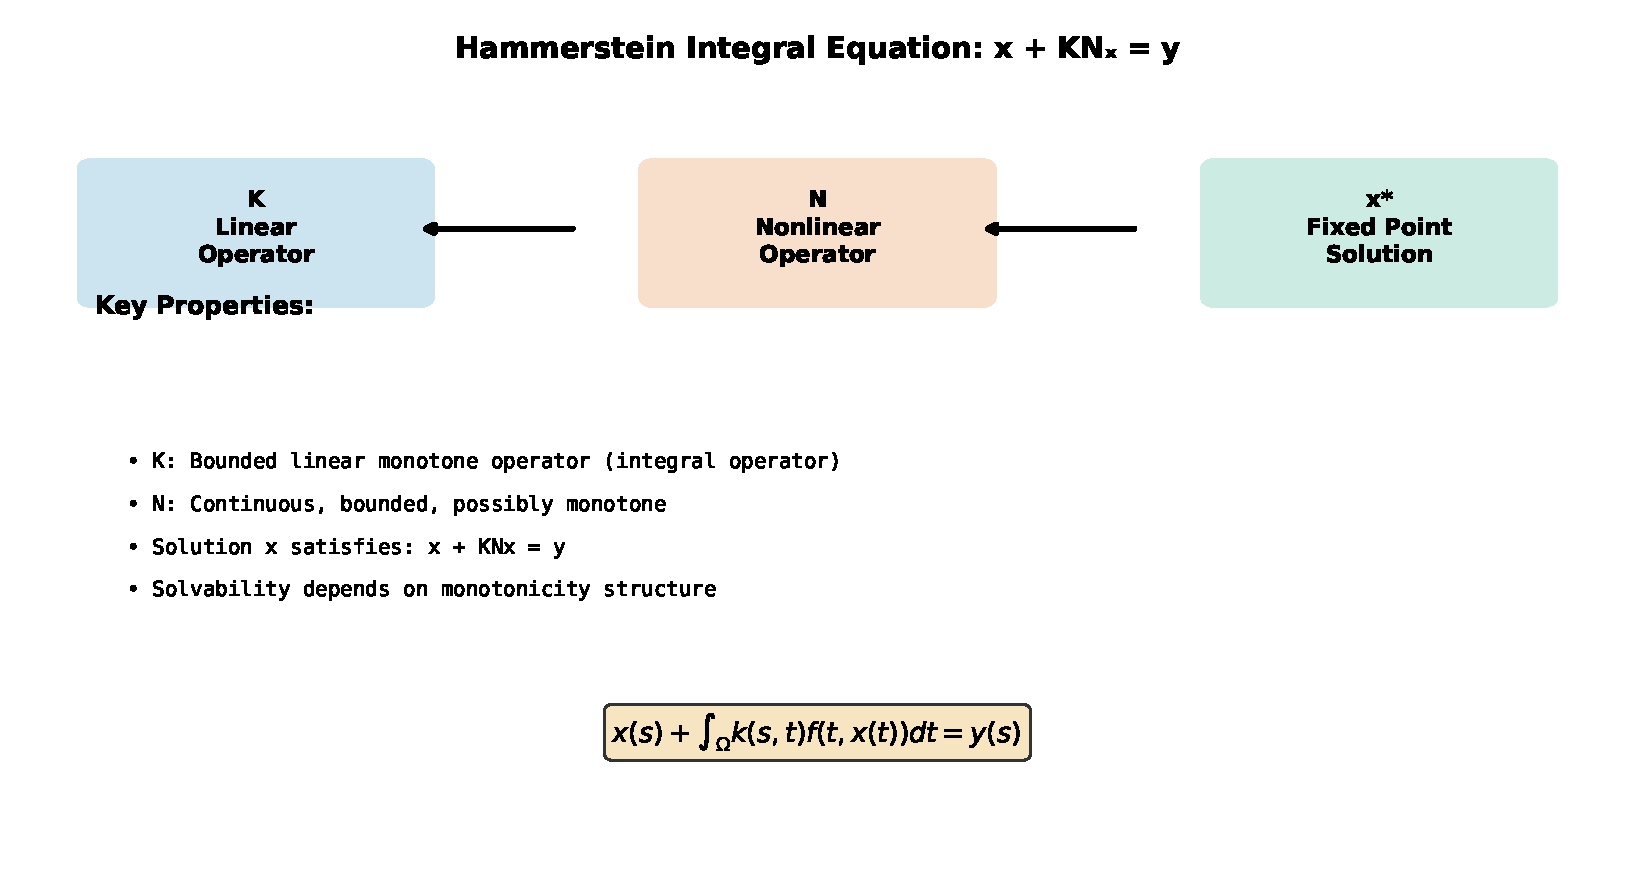
\includegraphics[width=\textwidth]{hammerstein_equation_schematic.pdf}
\end{frame}

\begin{frame}{Example 8.6: Concrete Hammerstein Equation}
    \begin{exampleblock}{Specific Hammerstein Problem}
        Consider the equation:
        \[
            x(s) + \int_{\Omega} k(s,t) f(t, x(t)) dt = 0
        \]
        with conditions:
        \begin{enumerate}
            \item $k(s,t)$ is symmetric, positive semidefinite, Hilbert-Schmidt kernel
            \item $f(s,x)$ is monotone increasing in $x$ with growth condition: $|f(s,x)| \leq a(s) + b|x|$
            \item For large $|x|$: $f(s,x) > a + bx$ (for $x > M$) or $f(s,x) < -a + bx$ (for $x < -M$)
        \end{enumerate}
    \end{exampleblock}

    \vspace{0.2cm}

    \textbf{Result:} This is equivalent to $x + KN_f x = 0$, and has a solution in $L_2(\Omega)$
    by Theorem 8.9, because $K$ is monotone and $N_f$ satisfies the coercivity condition.
\end{frame}

\begin{frame}[fragile]{Numerical Example: Solving Hammerstein Equation}{Python Implementation}
    \begin{lstlisting}
import numpy as np
from scipy.integrate import quad
from scipy.optimize import fsolve

# Hammerstein equation parameters
def hammerstein_kernel(s, t):
    """Symmetric kernel: k(s,t) = exp(-|s-t|)"""
    return np.exp(-np.abs(s - t))

def nonlinear_term(t, x_t):
    """Nonlinear operator: f(t, x) = tanh(x)"""
    return np.tanh(x_t)

def hammerstein_operator(x_vals, s_eval):
    """Compute integral term of Hammerstein equation"""
    result, _ = quad(lambda t: hammerstein_kernel(s_eval, t) *
                     nonlinear_term(t, np.interp(t, s_pts, x_vals)),
                     0, 1)
    return result

# Domain discretization
s_pts = np.linspace(0, 1, 21)
x_init = np.zeros_like(s_pts)

# Define the operator equation: x + K(Nf(x)) = 0
def operator_eq(x_vals):
    return [x_vals[i] + hammerstein_operator(x_vals, s_pts[i])
            for i in range(len(s_pts))]

# Solve using fixed point iteration
x_solution = fsolve(operator_eq, x_init)
    \end{lstlisting}

    The monotone structure ensures convergence and uniqueness of the solution.
\end{frame}

% ==================== SECTION 4: GENERALIZATIONS ====================
\section{Generalizations and Extensions}

\begin{frame}{Generalized Hammerstein Equations}
    \begin{definition}[Generalized Hammerstein Equation]
        The integral equation:
        \[
            u(s) + \int_{\Omega} k(s, t, u(t)) f(t, u(t)) dt = v(s)
        \]
        where the kernel $k(s,t,u)$ depends on the solution $u$.
    \end{definition}

    \vspace{0.3cm}

    \textbf{Operator form:} $u + K(u) N_f u = v$

    \vspace{0.3cm}

    \begin{theorem}[Theorem 8.17: Generalized Equations]
        Let $X$ be a reflexive Banach space and for each $u \in X$:
        \begin{itemize}
            \item $K(u): X^* \to X$ is angle-bounded with constant $c \geq 0$
            \item $u \mapsto K(u)$ is continuous from $X$ to $L(X^*, X)$
            \item $\|K(u)\| \leq r$ for all $u \in X$
        \end{itemize}
        If $N_f: X \to X^*$ is continuous, bounded, and $(u_1 - u_2, N_f u_1 - N_f u_2) \geq -k\|u_1 - u_2\|^2$ with $kr < (1+c^2)$,\\
        then $u + K(u)N_f u = 0$ has at least one solution.
    \end{theorem}
\end{frame}

\begin{frame}{Equations with Sum of Hammerstein Operators}
    \begin{problem}[Mixed Type Integral Equation]
        \[
            u(s) + \int_{\Omega} K_1(s,t) f_1(t, u(t)) dt + \int_{\Omega} K_2(s,t) f_2(t, u(t)) dt = 0
        \]
    \end{problem}

    \vspace{0.3cm}

    \textbf{Operator form:} $u + K_1 N_1 u + K_2 N_2 u = 0$

    \vspace{0.3cm}

    \textbf{Key approach:}
    \begin{enumerate}
        \item Define the product Banach space: $\X = X \times X \times \cdots \times X$
        \item Define composite linear operator $K: \X \to \X^*$
        \item Define composite nonlinear operator $N: \X \to \X^*$
        \item Apply theorems to the combined equation
    \end{enumerate}

    \vspace{0.3cm}

    This allows handling systems of coupled integral equations through a unified framework.
\end{frame}

\begin{frame}{Urysohn's Integral Equation}
    \begin{definition}[Urysohn's Integral Equation]
        An integral equation where $f$ depends on both $t$ and $x(t)$:
        \[
            x(s) + \int_{\Omega} k(s, t, x(t)) dt = y(s)
        \]
    \end{definition}

    \vspace{0.3cm}

    \textbf{Characteristics:}
    \begin{itemize}
        \item More general than Hammerstein (kernel depends on solution)
        \item Classical problem in nonlinear analysis
        \item Can be treated using monotone operator methods
        \item Often requires Leray-Schauder principle for existence
    \end{itemize}

    \vspace{0.3cm}

    \textbf{Remark:} The monotone operator approach unifies treatment of different integral equation types through operator-theoretic perspective rather than specialized techniques for each type.
\end{frame}

% ==================== SECTION 5: COMPUTATIONAL METHODS ====================
\section{Computational Methods and Convergence}

\begin{frame}{Iterative Methods for Hammerstein Equations}
    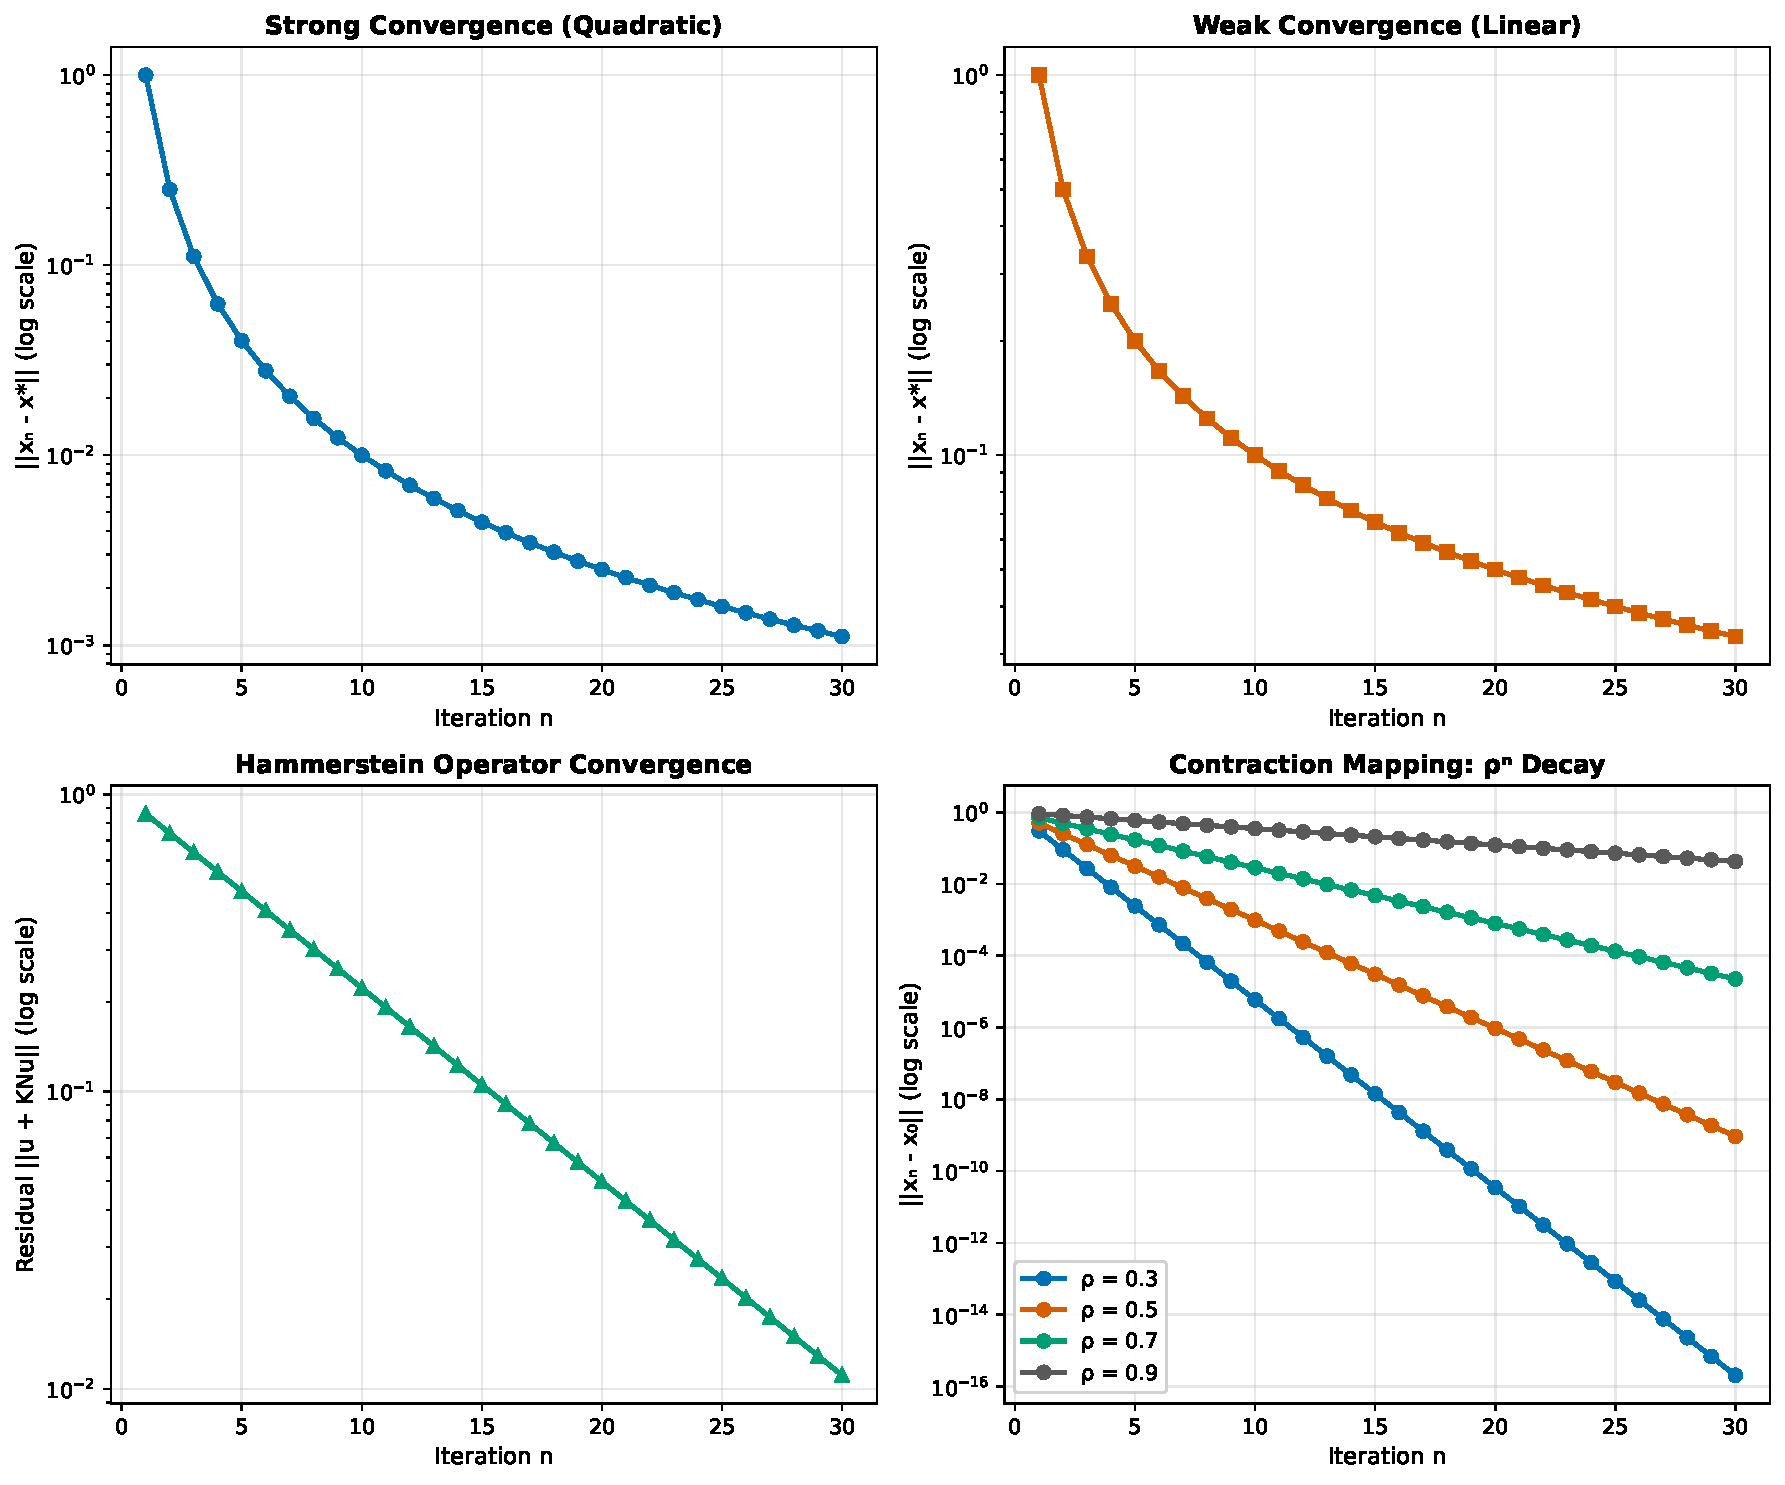
\includegraphics[width=\textwidth]{iterative_convergence.pdf}
\end{frame}

\begin{frame}[allowframebreaks]{Bruck's Jr. Iterative Scheme}
    \begin{theorem}[Theorem 8.21: Iterative Solution]
        Let $X$ be a reflexive Banach space and $K: X \to X^*$ a symmetric, monotone, bounded linear operator.
        Let $N: X^* \to X$ be a nonlinear hemicontinuous operator satisfying:
        \[
            \langle u_1 - u_2, Nu_1 - Nu_2 \rangle \geq -k\|u_1 - u_2\|_{\mathcal{X}^*}^2
        \]

        If $k\|K\| < 1$, then $u + KNu = w$ has a unique solution $u \in X$, and the sequence
        defined by Bruck's scheme:
        \[
            v_{n+1} = \frac{n}{n+1}v_n - \frac{1}{n+1}SN[S^*v_n + w]
        \]
        converges to the solution with convergence rate $\|S^*v_n + w - u\| = O(n^{-1/2})$.
    \end{theorem}

    \framebreak

    \textbf{Key Components:}
    \begin{itemize}
        \item $S: X \to \HH$ is a continuous linear mapping
        \item $\HH$ is a Hilbert space with $S^*$ injective
        \item The splitting lemma provides the decomposition
        \item Averaging mechanism $\frac{n}{n+1}v_n$ ensures convergence
    \end{itemize}

    \vspace{0.3cm}

    \textbf{Practical advantages:}
    \begin{enumerate}
        \item Guaranteed convergence under verifiable conditions
        \item Convergence rate $O(n^{-1/2})$ is optimal for this class
        \item Applicable to wide range of nonlinear integral equations
    \end{enumerate}
\end{frame}

\begin{frame}{Computational Scheme: Hammerstein Operator Equations}
    \textbf{Algorithm: Iterative solver for $u + KNu = w$}

    \begin{enumerate}
        \item Initialize $v_1 \in \HH$ (arbitrary)
        \item For $n = 1, 2, \ldots, N_{\max}$:
        \begin{enumerate}
            \item Compute: $h_n = S^*v_n + w$
            \item Evaluate: $N(h_n)$ (nonlinear operator)
            \item Apply: $K(u_n) = K(N^{-1}v_n)P_n Nu_n$
            \item Update: $v_{n+1} = \frac{n}{n+1}v_n - \frac{1}{n+1}SN[S^*v_n + w]$
            \item If $\|v_{n+1} - v_n\| < \epsilon$, then break (convergence achieved)
        \end{enumerate}
        \item Recover: $u = S^*v_n + w$
    \end{enumerate}

    \vspace{0.3cm}

    \textbf{Convergence:} For $k(1 + c^2)\|K\| < 1$, guaranteed convergence with rate $O(n^{-1/2})$.
\end{frame}

\begin{frame}[fragile]{Numerical Example: Bruck's Iterative Scheme}{Python Implementation}
    \begin{lstlisting}
def brucks_iteration(K_operator, N_operator, w, x0, max_iter=500, tol=1e-6):
    """
    Bruck Jr. iterative scheme for u + K*N(u) = w
    Returns iterates and convergence history
    """
    residuals = []
    u_vals = [x0]

    for n in range(1, max_iter):
        # Apply nonlinear operator
        N_u = N_operator(u_vals[-1])

        # Apply linear operator: K*N(u)
        K_N_u = K_operator(N_u)

        # Compute residual and update
        residual = np.linalg.norm(u_vals[-1] + K_N_u - w)
        residuals.append(residual)

        # Bruck iteration: averaging
        u_next = (n / (n + 1)) * u_vals[-1] - \
                 (1 / (n + 1)) * K_N_u

        u_vals.append(u_next)

        if residual < tol:
            print(f"Converged at iteration {n}")
            break

    return np.array(u_vals), np.array(residuals)

# Apply to Hammerstein equation
u_solution, residuals = brucks_iteration(K_op, N_op, w, u_init)
    \end{lstlisting}
\end{frame}

% ==================== SECTION 6: NORMAL STRUCTURE AND FIXED POINTS ====================
\section{Normal Structure and Fixed Point Theorems}

\begin{frame}{Banach Space Properties}
    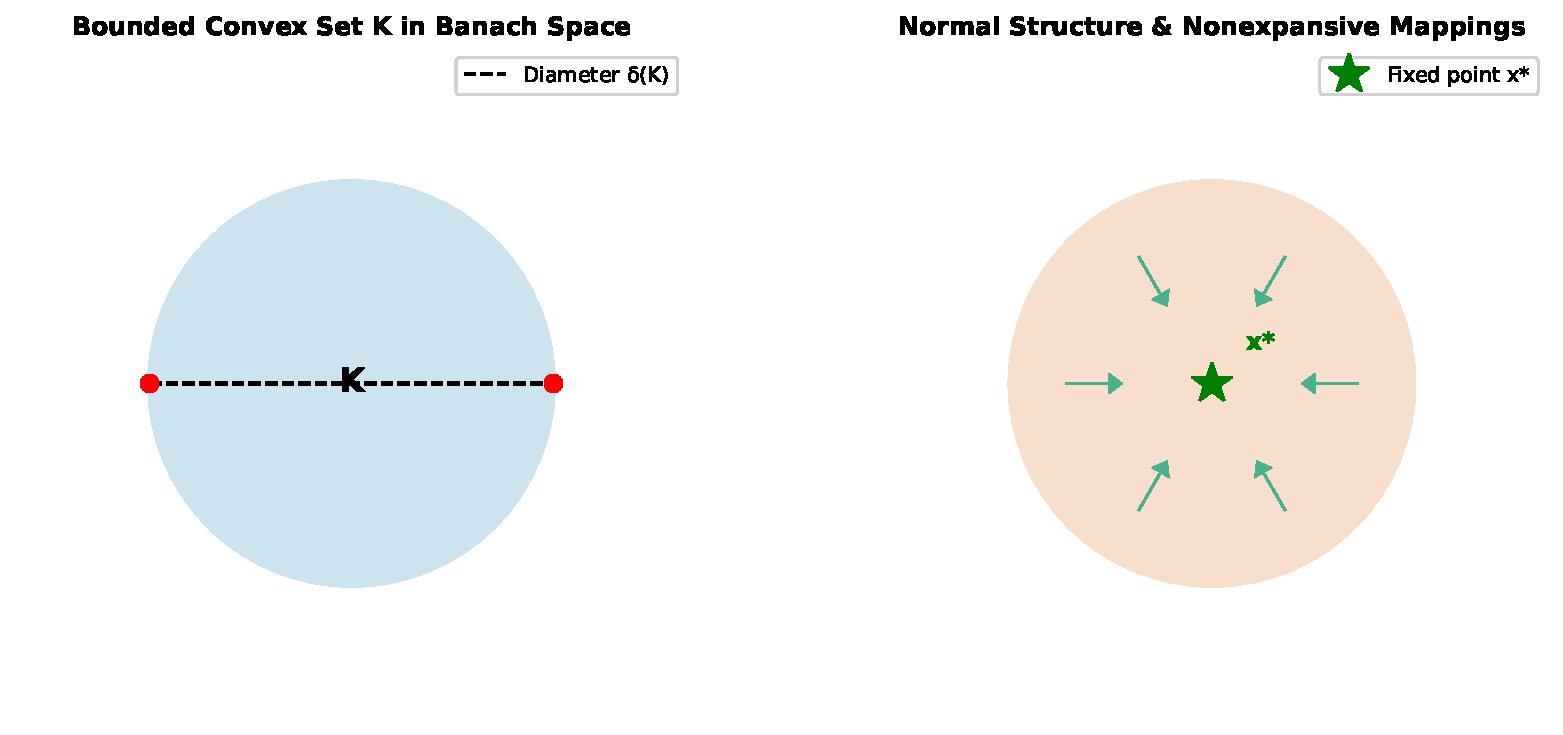
\includegraphics[width=\textwidth]{banach_space_normal_structure.pdf}
\end{frame}

\begin{frame}{Kirk's Theorem and Normal Structure}
    \begin{theorem}[Kirk's Fixed Point Theorem]
        Let $K$ be a bounded convex set in a Banach space $X$ with normal structure,
        and let $F: K \to K$ be a nonexpansive mapping
        (i.e., $\|Fx - Fy\| \leq \|x - y\|$ for all $x, y \in K$).\\
        Then $F$ has a fixed point in $K$.
    \end{theorem}

    \vspace{0.3cm}

    \textbf{Key observations:}
    \begin{itemize}
        \item Normal structure is more general than compactness
        \item Includes unbounded but non-trivial convex sets
        \item Equivalence with reflexivity + weak lower semicontinuity properties
        \item Uniformly convex spaces automatically have normal structure
    \end{itemize}

    \vspace{0.3cm}

    \begin{corollary}
        If $K$ has normal structure and $F: K \to K$ is nonexpansive, then $\delta(K_0) < \delta(K)$
        for any closed convex subset $K_0 \neq K$ that is invariant under $F$.
    \end{corollary}
\end{frame}

\begin{frame}{Concept Hierarchy}
    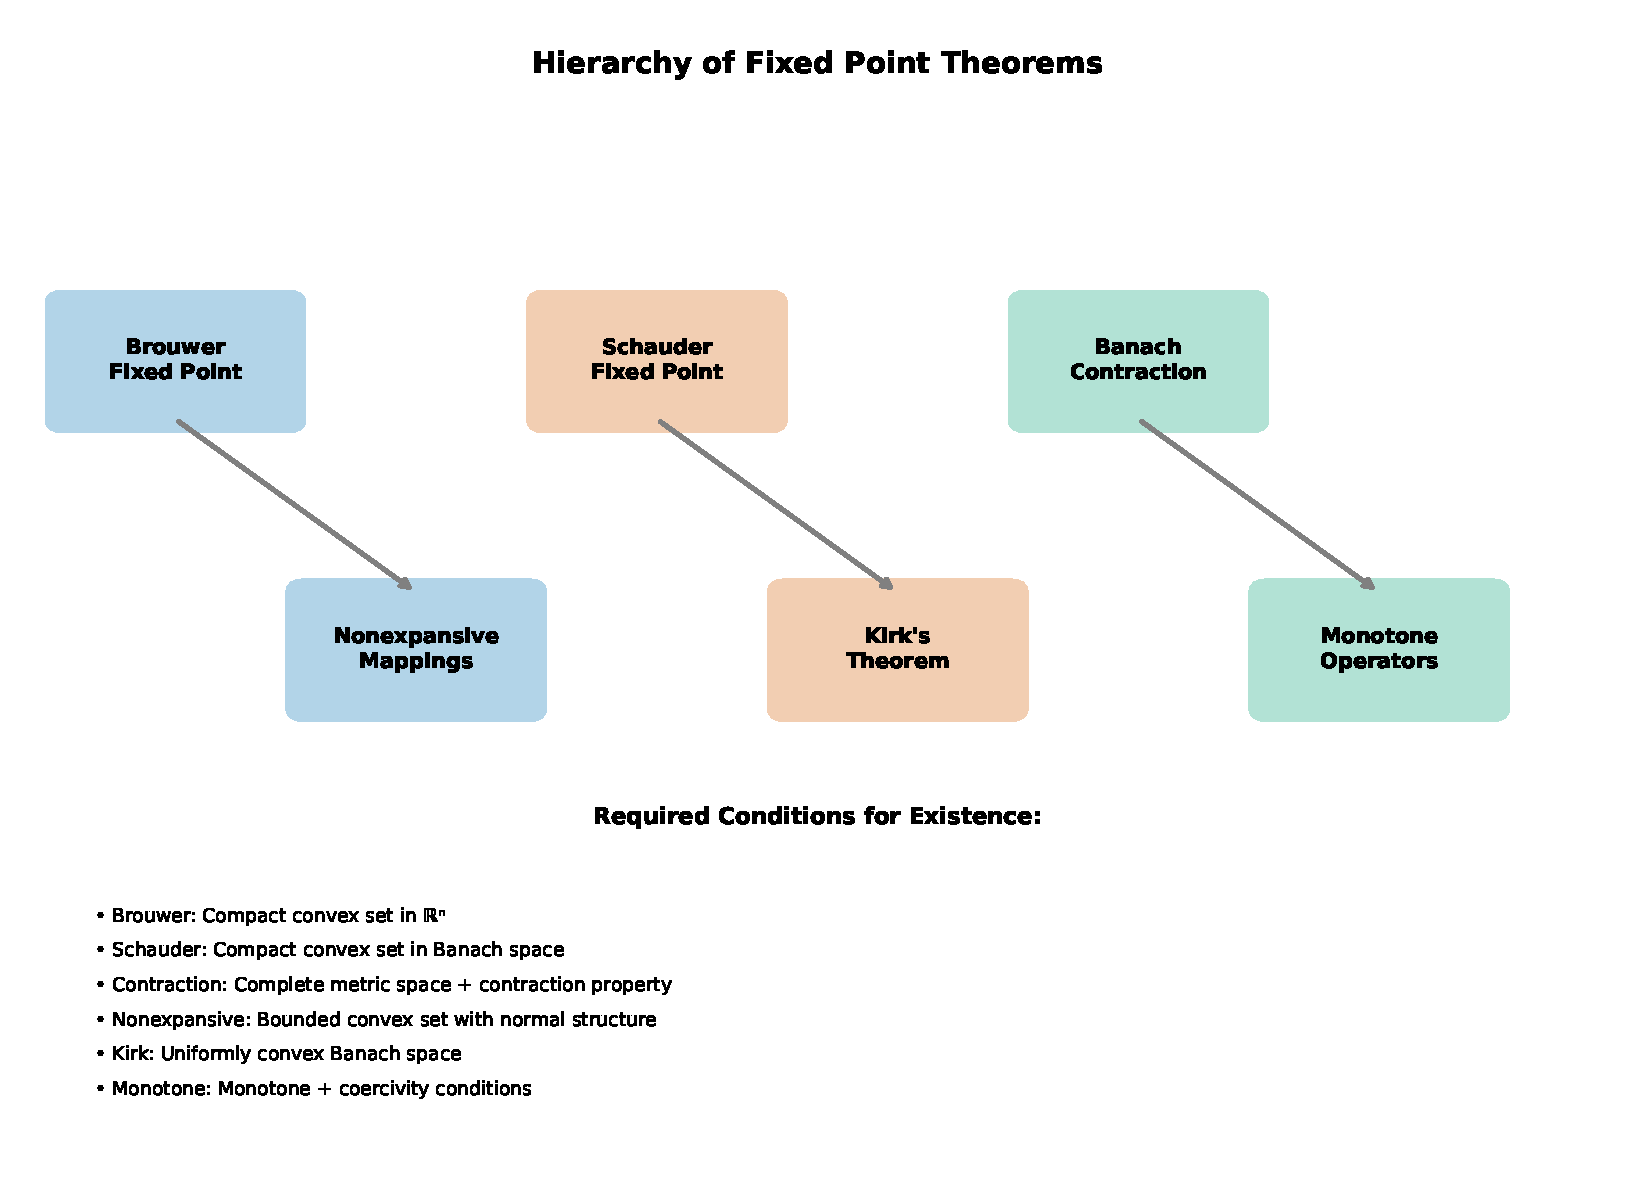
\includegraphics[width=\textwidth]{fixed_point_theorem_hierarchy.pdf}
\end{frame}

\begin{frame}{Uniformly Convex Spaces}
    \begin{definition}[Uniformly Convex]
        A Banach space $X$ is \textbf{uniformly convex} if for every $\epsilon > 0$,
        there exists $\delta > 0$ such that:
        \[
            \left\| \frac{x + y}{2} \right\| > 1 - \delta \quad \text{whenever } \|x\| = \|y\| = 1, \, \|x - y\| \geq \epsilon
        \]
    \end{definition}

    \vspace{0.3cm}

    \textbf{Equivalent characterizations:}
    \begin{itemize}
        \item The norm is strictly convex
        \item Every bounded sequence has at most one weak limit point
        \item If $x_n \rightharpoonup x$ and $\|x_n\| \to \|x\|$, then $x_n \to x$ (norm convergence)
    \end{itemize}

    \vspace{0.3cm}

    \begin{theorem}
        Every uniformly convex Banach space is reflexive, and thus has normal structure.
    \end{theorem}

    \vspace{0.3cm}

    \textbf{Examples:} $L^p$ spaces with $1 < p < \infty$, Sobolev spaces $W^{1,p}$ with $1 < p < \infty$.
\end{frame}

% ==================== SECTION 7: SUMMARY AND APPLICATIONS ====================
\section{Summary and Applications}

\begin{frame}{Main Results Summary}
    \begin{center}
        \begin{tabular}{|c|c|c|}
            \hline
            \textbf{Problem Class} & \textbf{Operator Structure} & \textbf{Existence Tool} \\
            \hline
            Hammerstein Eq. & $x + KN_f x = y$ & Monotone $K$ + Hemicontinuous $N_f$ \\
            \hline
            Generalized Ham. & $u + K(u)N_f u = v$ & Angle-bounded $K(u)$ \\
            \hline
            Mixed Type & $u + \sum_j K_j N_j u = 0$ & Product space structure \\
            \hline
            Urysohn Eq. & $x + \int k(s,t,x(t))dt = y$ & Kernel monotonicity \\
            \hline
            Fixed Points & $F(x) = x$ in $K$ & Normal structure \\
            \hline
        \end{tabular}
    \end{center}

    \vspace{0.5cm}

    \textbf{Unifying principle:} Monotone operators and normal structure provide
    geometric and analytical tools for existence and uniqueness results across different problem classes.
\end{frame}

\begin{frame}{Application Domains}
    \textbf{1. Nonlinear Differential Equations:}
    \begin{itemize}
        \item Boundary value problems as integral equations
        \item Coupled systems of PDEs
    \end{itemize}

    \vspace{0.2cm}

    \textbf{2. Nonlinear Integral Equations:}
    \begin{itemize}
        \item Hammerstein equations from integral operators
        \item Volterra and Fredholm type problems
    \end{itemize}

    \vspace{0.2cm}

    \textbf{3. Nonlinear Optimization:}
    \begin{itemize}
        \item Variational inequalities
        \item Monotone inclusion problems: $0 \in A(x)$
    \end{itemize}

    \vspace{0.2cm}

    \textbf{4. Applied Mathematics:}
    \begin{itemize}
        \item Heat radiation transfer (Chandrasekhar's equation)
        \item Fluid mechanics (Navier-Stokes type problems)
        \item Control theory (optimal control formulations)
    \end{itemize}

    \vspace{0.2cm}

    \textbf{5. Computational Methods:}
    \begin{itemize}
        \item Fixed point iterations with guaranteed convergence
        \item Iterative schemes with convergence rates
    \end{itemize}
\end{frame}

\begin{frame}{Open Problems and Extensions}
    \begin{itemize}
        \item \textbf{Weak convergence:} Characterize spaces where weak convergence sequences have fixed points

        \vspace{0.2cm}

        \item \textbf{Non-compact operators:} Develop theory for condensing maps and measures of noncompactness

        \vspace{0.2cm}

        \item \textbf{Nonlinear semigroups:} Evolution equations with monotone operators

        \vspace{0.2cm}

        \item \textbf{Variational methods:} Mountain pass theorems and critical points

        \vspace{0.2cm}

        \item \textbf{Computational aspects:} Optimal convergence rates and algorithmic improvements
    \end{itemize}

    \vspace{0.3cm}

    These extensions connect to variational principles, degree theory, and topological methods
    discussed in subsequent chapters.
\end{frame}

\begin{frame}[allowframebreaks]{References and Further Reading}
    \small

    \textbf{Primary Source:}
    \begin{itemize}
        \item Pathak, H. K. (2018). \textit{An Introduction to Nonlinear Analysis and Fixed Point Theory}.
              Springer. Chapter 6-8.
    \end{itemize}

    \vspace{0.3cm}

    \textbf{Classical References:}
    \begin{itemize}
        \item Dolph, C. L., \& Minty, G. J. (1964). On nonlinear integral equations of the Hammerstein type.
              \textit{Nonlinear Integral Equations}.

        \item Kirk, W. A. (1965). A fixed point theorem for mappings which do not increase distances.
              \textit{American Mathematical Monthly}.

        \item Krasnosel'skii, M. A. (1964). \textit{Topological Methods in the Theory of Nonlinear Integral Equations}.
    \end{itemize}

    \vspace{0.3cm}

    \textbf{Modern Approaches:}
    \begin{itemize}
        \item Brezis, H. (2011). \textit{Functional Analysis, Sobolev Spaces and Partial Differential Equations}.

        \item Zeidler, E. (1990-1995). \textit{Nonlinear Functional Analysis and its Applications} (Vol. I-V).

        \item Bauschke, H. H., \& Combettes, P. L. (2017). \textit{Convex Analysis and Monotone Operator Theory}.
    \end{itemize}

    \framebreak

    \textbf{Related Topics:}
    \begin{itemize}
        \item Leray-Schauder degree theory for existence proofs
        \item Condensing maps and measures of noncompactness
        \item Asymptotic behavior of iterative sequences
        \item Applications to PDEs and integral equations
    \end{itemize}
\end{frame}

% Final slide
\begin{frame}
    \centering
    \Large
    \textbf{Thank you!}\\[1cm]
    Questions and Discussion
\end{frame}

\end{document}
